\documentclass[11pt]{article}
% default ORG mode 
\usepackage[utf8]{inputenc}  \usepackage[T1]{fontenc} \usepackage{fixltx2e}
\usepackage{graphicx}        \usepackage{longtable}   \usepackage{float}
\usepackage{wrapfig}         \usepackage{soul}        \usepackage{textcomp}
\usepackage{marvosym}        \usepackage{wasysym}     \usepackage{latexsym}
\usepackage{amsmath}         \usepackage{amssymb}     \usepackage{color}
\usepackage{rotating}        \usepackage{hyperref}    \usepackage{xcolor} 
\usepackage{palatino}
% my customizations
\usepackage{enumitem}
\usepackage{amsthm}
\tolerance=1000
%\providecommand{\alert}[1]{\textbf{#1}}
\usepackage[top=1in, bottom=1in, left=1in, right=1in]{geometry}

\title{Dodson \& Poston Exercise VII.1.7}
\author{Peter Mao, $\ldots$}
\date{\today}

\begin{document}

\maketitle
\pagestyle{empty}

\begin{abstract}
  In-progress solution.  Feel free to add/comment/disparage.  See Randy's solution.
\end{abstract}



\begin{itemize}
\item[\textbf{(a)}] Use $f(x) = x^3$ to show that the ``if'' of Corollary 1.05
  cannot be strengthened to ``iff''.
\item[\emph{Solution}] Corollary 1.05 states that if $f$ is $C^1$ and $D_xf$ is
  injective, then there is a neighborhood of $x$, $N$, such that $f|_N$ is
  injective.  In the example given, $f$ is $C^1$ and $f|_N$ is injective for any
  neighborhood of any $x$, but $D_0f$ is not injective, providing a
  counterexample to the ``only if'' part of ``iff''.
  

\item[\textbf{(b)}]
\item[\emph{Solution}] See Figure~\ref{fig:7b}
  \begin{figure}[h]
    \centerline{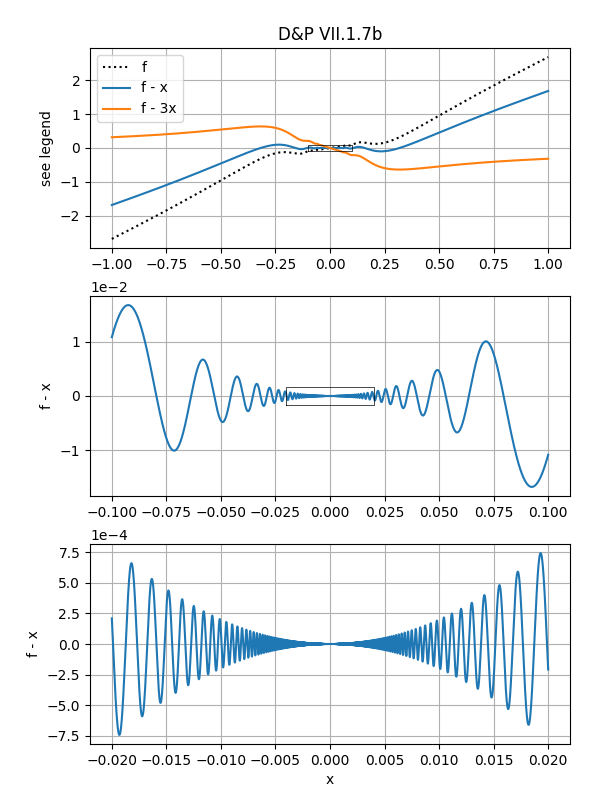
\includegraphics[height=7in]{figs/Ex.VII.1.7b.png}}
    \caption{\textbf{Top}: $\protect f$, $\protect f-x$ and $\protect f-3x$ over
      the range [-1,1].  Near $\protect x=0$, the salient features of f are best
      shown by f-x.  Far from $\protect x=0$, the slope of f asymptotes to 3
      (hence the $\protect f-3x$).  \textbf{Middle}: $\protect f-x$ over the
      range [-0.1,0.1].  The main features of $\protect f$ start to become
      evident at this range -- diminishing of both amplitude and wavelength as x
      approaches 0. \textbf{Bottom}: At all smaller ranges in $\protect x$, the
      picture is the same -- a parabolic envelope and ever shortening wavelength
      as $\protect x \rightarrow 0$.  Although the slope of $\protect f$
      approaches 1 as $\protect x \rightarrow 0$, it approaches the asymptotic
      slope from both above and below the limiting value. }
    \label{fig:7b}
  \end{figure}


\item[\textbf{(c)}]
\item[\emph{Solution}]
  
\end{itemize}
\end{document}



%% commonly used blocks
\begin{quote}
\end{quote}

\begin{proof}
\end{proof}

\begin{align}
\end{align}

\begin{equation}
\end{equation}

\begin{remark}
\end{remark}

